\documentclass[a4paper,11pt,titlepage,drop]{article}%
\usepackage{graphicx}
\usepackage{xspace}
%%\usepackage[section]{placeins}
%\usepackage[caption=false]{subfig}
\usepackage{amsmath}%
\usepackage{amsfonts}%
\usepackage{amssymb}%
\usepackage[english,oldcommands,plain,lined]{algorithm2e}
\usepackage{graphicx} \DeclareGraphicsExtensions{.png,.jpg,.eps}   %%% standard extension for included graphics
\usepackage{graphics}
\usepackage{setspace}
\usepackage[left=1.5in,top=1in,right=1in,bottom=1in]{geometry}
\usepackage{subfigure}    %% For putting multiple figures together.
\usepackage{makeidx}      %% creating index
\usepackage{nomencl}	  %% For list of abbreviations
\usepackage{appendix}	  %% For creating Appendix
\usepackage{html}
\usepackage{url}
\usepackage{hyperref}
\hypersetup{
  colorlinks=true,
  linkcolor=blue,
  citecolor=magenta
}
%usepackage[colorlinks=true,linkcolor=blue,citecolor=magenta]{hyperref}
	\def\sectionautorefname{Section}
	\def\chapterautorefname{Chapter}
	\def\figureautorefname{Figure}
	\def\subfigureautorefname{Figure}
%\usepackage[backend=bibtex,bibstyle=authoryear,citestyle=authoryear,sorting=nyt,maxbibnames=99,maxcitenames=3]{biblatex}
%\bibliography{report}
\usepackage[dcucite,abbr]{harvard}
\usepackage{lettrine}
\usepackage[T1]{fontenc}
\usepackage{multirow}
\usepackage{rotating}
\usepackage{times}
\usepackage{float}
\usepackage{wasysym}
\usepackage{lineno}
\usepackage[normalem]{ulem}
\usepackage{tfrupee}
\usepackage{amsmath}
\usepackage[official]{eurosym}
\usepackage{graphicx}
\usepackage [english]{babel}
\usepackage{amsmath}  
\usepackage [autostyle, english = american]{csquotes}
\newcommand\etc{\emph{etc.}}
\newcommand\viz{\emph{viz.}}
\newtheorem{theorem}{Theorem}
\newtheorem{acknowledgement}[theorem]{Acknowledgement}
\newtheorem{axiom}[theorem]{Axiom}
\newtheorem{case}[theorem]{Case}
\newtheorem{claim}[theorem]{Claim}
\newtheorem{conclusion}[theorem]{Conclusion}
\newtheorem{condition}[theorem]{Condition}
\newtheorem{conjecture}[theorem]{Conjecture}
\newtheorem{corollary}[theorem]{Corollary}
\newtheorem{criterion}[theorem]{Criterion}
\newtheorem{definition}[theorem]{Definition}
\newtheorem{example}[theorem]{Example}
\newtheorem{exercise}[theorem]{Exercise}
\newtheorem{lemma}[theorem]{Lemma}
\newtheorem{notation}[theorem]{Notation}
\newtheorem{problem}[theorem]{Problem}
\newtheorem{proposition}[theorem]{Proposition}
\newtheorem{remark}[theorem]{Remark}
\newtheorem{solution}[theorem]{Solution}
\newtheorem{summary}[theorem]{Summary}
\newenvironment{proof}[1][Proof]{\textbf{#1.} }{\ \rule{0.5em}{0.5em}}


\newenvironment{citemize}{
	\begin{itemize}
		\setlength{\itemsep}{1pt}
		\setlength{\parskip}{0pt}
		\setlength{\parskip}{0pt}}
{\end{itemize}}

\newenvironment{cenumerate}{
	\begin{enumerate}
		\setlength{\itemsep}{1pt}
		\setlength{\parskip}{0pt}
		\setlength{\parskip}{0pt}}
{\end{enumerate}}

\begin{document}

\bibliographystyle{dcu}

\thispagestyle{empty}

\begin{center}
    \Huge\bfseries
    Learning to Predict Driving States using Generative Adversarial Networks and Dashboard Mounted Multiple Sensors towards Autonomous Driving Assistance
\end{center}

\vfill \vfill \vfill \vfill

\begin{center}
    \bfseries
    Thesis Report Submitted in Partial Fulfillment \\ of the Requirements for the Award of the Degree of 
\end{center}

\vfill

\begin{center}
    \Large\bfseries
    Bachelor of Technology
\end{center}

\vfill

\begin{center}
    \bfseries
    by
\end{center}

\vfill

\begin{center}
    \Large\bfseries
    Rahul Kumar Singh \\
     \large\bfseries 
     13EE10065 \\
\end{center}

\vfill

\begin{center}
    \bfseries
    Under the supervision of
\end{center}

\vfill

\begin{center}
    \Large\bfseries
    Dr. Debdoot Sheet \\
     \large\bfseries 
\end{center}

\vfill \vfill \vfill \vfill

\begin{figure}[h]
\centering

\includegraphics[width=1.31in,height=1.42in]{kgp}
\end{figure}

\begin{center}
    \Large\bfseries
    Department of Electrical Engineering\\
    Indian Institute of Technology Kharagpur \\
    December 2016
\end{center}
%%%%%%%%%%%%%%%%%%%%%%%%%%%%%%%%%%%%%%%%%%%%%%%%%%%%%%%%%%%%%%%%%%
%%%%%%%%%%%%%%%%%%%%%%%%%%%%%%%%%%%%%%%%%%%%%%%%%%%%%%%%%%%%%%%%%%
%\newpage
%\thispagestyle{empty}
%
%\begin{center}
%    \Huge\bfseries
%    Certificate
%\end{center}
%
%
%
%\begin{flushleft}
%This is to certify that the B.Tech project entitled "\textbf {\textit{Learning to Predict Driving Activities using Generative Adversarial Networks and Dashboard Mounted Multiple Sensors towards Autonomous Driving Assistance}}", which has been submitted by  \textbf{Rahul Kumar Singh (13EE10065)}, is a bonafide work carried out by him under our supervision and guidance. It is worthy of consideration for the partial requirement for the award of the degree Bachelor of Technology in Electrical Engineering by the Indian Institute of Technology Kharagpur. 
%\end{flushleft}
%
%\vfill
%
%
%
%\begin{center}
%\begin{tabular}{ c c c c }
% \large\bfseries Prof. Debdoot Sheet \\ 
% \normalsize\bfseries Department of Electrical Engineering \\ 
%   \normalsize\bfseries IIT Kharagpur 
%\end{tabular}
%\end{center}
%
%\vfill
%\vfill \vfill \vfill \vfill
%%%%%%%%%%%%%%%%%%%%%%%%%%%%%%%%%%%%%%%%%%%%%%%%%%%%%%%%%%%%%%%%%
%%%%%%%%%%%%%%%%%%%%%%%%%%%%%%%%%%%%%%%%%%%%%%%%%%%%%%%%%%%%%%%%%

\newpage
\thispagestyle{empty}
\onehalfspacing

\section*{Abstract}

Autonomous driving in cars are gaining a centre-stage, as prospects of the future is triggering significant research in the machine learning and vision community. Research areas for autonomous car driving range from predicting driving trajectory to predictive simulation of driving conditions and generation of large multi-sensor datasets along with preparing benchmarks of autonomous drivability tests for special hardware-software suite development to facilitate such research. In order to  make a conventional fuel based car with an internal combustion engine autonomous, we generally would like to control the gas pedal (accelerator), clutch, gear lever, brake pedal and the steering wheel based on driving condition inputs from car mounted cameras, light detection and ranging (LIDAR), radio detection and ranging (RADAR), accelerometer, gyroscope, magnetometer and GPS sensors. In this project, we are currently extending on the prior art for predictive modeling of the other driving states like gas pedal (accelerator), clutch, gear lever, brake pedal press using multi-sensor integration for modeling of these states. The publicly available driving dataset consisting of 7.25 hours of highway rich quality video feed with other sensor data like speed, acceleration, 3D LIDAR along with car driving control variable data for the training. Currently we have implemented the steering angle predicting by training on 9 videos set and predicting on 2 videos sets to obtain a MSE of $\mathbf{1\times10^{-2}}$


\vskip 2in

\noindent\textbf{\textit{Keywords:}} Autonomous driving, autoencoder, convolutional neural networks, driving state estimation, long-short term memory, transfer learning, temporal modelling.

\newpage

\singlespacing

\setcounter{tocdepth}{2}
\thispagestyle{empty}
\tableofcontents
\newpage

\setcounter{page}{1}

\onehalfspacing

%\linenumbers
%\renewcommand\thelinenumber{\color{red}\arabic{linenumber}}

% INTRODUCTION
\section{Introduction}

\lettrine{A}{utonomous} cars are future of mobility and field of deep learning \cite{deep} is helping in paving a way for solving core problems associated with it. Many automobile companies as well as scientific groups around the world are actively working in this field. Companies like \href{http://www.nvidia.com/object/drive-automotive-technology.html}{NVidia}\footnote{http://www.nvidia.com/object/drive-automotive-technology.html} \cite{nvidia}, Ford, Tesla \cite{tesla}, BMW \footnote{http://www.bmw. com/com/en/insights/technology/connecteddrive/ 2010/future} are competing on global scale while companies like comma.ai\footnote{http://research.comma.ai/}, appleare developing software tools for autonomous cars. Car driving conditions are generally grouped as dense urban journey and initiate/terminate conditions when speed ranges in 0-10 kmph and is good for real-time processing in any environment, but with high dynamics in the environment where  travel speed varies from 10 to 50 kmph with lots of unpredictability in the driving environment makes it quite challenging to model; however,cruising speeds of 50-100 kmph on the highways where less unpredictability of driving conditions assists in less challenging situations to model.

Car driving is a set of skills which requires controlling steering, transmission (gear, gas) and break. An autonomous car requires prediction of these driving states given the input from the sensors. Traditionally, approach towards self-driving cars was driven more in complexly coded structure which accounted enormous number of possibilities which can occur during driving. Vision has been an important sensory data which has been employed in self-driving cars \cite{stanford}. But, it becomes nearly difficult to code the highly dynamic and complex vehicular environment from visual data. The recent growth of research in deep learning has led to a paradigm shift in the approach for self-driving cars. Earlier, more time was consumed in analysis of different situations (implementation of multiple algorithms) which prevented real-time implementation. Now, the trend has shifted, i.e. more time is spent during training while minimizing the time at the time of testing. With powerful GPUs coming in (NVidia e.g.), parallelism and computation hungry task are dealt more efficiently.

Deep learning uses the property that many natural images are constituted in a hierarchial order and the neighbouring pixels are highly correlated. The hierarchincal order consists of high level features like square consisting of sub low level features like egdes, lines. New deep learning techniques like Convolutional Neural Networks (CNNs), Recurrent Neural Networks (RNNs), Auto encoders and their variants have helped in modeling complex sensory rich data and generate useful commands. Lot of research is being done is this field where variety of techniques using combination of these networks is being used. \citeasnoun{lrcn} have used long-term recurrent convolutional network for visual recognition and description task while \cite{inteldrive1} used neural networks for modelling driver behaviour and \cite{inteldrive2} has used driving style recognition for improving driving efficiency by increasing the battery performance of a hybrid vehicle. These techniques are data centric i.e. convergence is very much dependent on input data. Many open source datasets are  available \href{http://www.cvlibs.net/datasets/kitti/}{kitty} \cite{kitty}, \href{http://research.comma.ai/}{comma.ai} and \href{https://github.com/udacity/self-driving-car/tree/master/datasets}{udacity}. These datasets are taken in urban environment on highways. 

Application of this techniques include path planning for semi-autonomous vehicles, efficient fuel usage in hybrid cars by minimizing the switching between fuel and battery. This will be useful in design of Self driving cars as vast dataset from human driving can be used to train the system to operate in different environmental and road conditions. 


% PRIOR ART  ~\cite{conv}
\section{Background}
\subsection{Autoencoder}

An autoencoder module consists of encoder and a decoder module. Encoder module converts a high dimensional data, for example, an image to a low dimensional latent space. Then the decoder module tries to reconstructs back the input data from the latent space. \citeasnoun{hinton} show any effective way of weight initialization for autoencoder training.  The encoder and the decoder can be defined as transitions $\phi$ and $\varphi$ respectively such that,
 
\begin{equation}
\label{eq:encoder}
\phi : \chi \xrightarrow{} 	\Theta
\end{equation}
\begin{equation}
		\label{eq:decoder}
					\varphi : \Theta  \xrightarrow{} \chi
\end{equation}
\begin{equation}
		\label{eq:error}
					\arg \min \limits_{\phi , \varphi} \parallel{X - (\phi \circ \varphi)X}\parallel^2				
\end{equation}

Eq. (\ref{eq:error}) determines mean squared error between input and reconstructed data is often used as a cost function assuming probability distribution of the error signal is Gaussian. In  (\ref{eq:encoder}), $\chi$ represents input space where as $\Theta$ represents the latent space. There are many variants of autoencoders for example sparse autoencoder \cite{ng}, denoising autoencoder \cite{denoise} and variational autoencoders \cite{autoen}.
 
\subsection{Convolutional Neural Networks} 

Convolutional networks are inspired by biological processes and are very similar to ordinary neural networks and been employed in many image classification tasks \cite{cnn} . They are made up of neurons that have learnable weights and biases. ConvNet architectures make the explicit assumption that the inputs are images, which allows us to encode certain properties into the architecture. Convolutional Neural Networks take advantage of the fact that the input consists of images and they constrain the architecture in a more sensible way. In particular, unlike a regular Neural Network, the layers of a ConvNet have neurons arranged in 3 dimensions: width, height, depth. Every layer of a ConvNet transforms the 3D input volume to a 3D output volume of neuron activations. CNNs are difficult to train as they typically contain a high number of unknowns.

\subsection{Long-Short Term Memory } 

In a traditional recurrent neural network, during the gradient back-propagation phase, the gradient signal can end up being multiplied a large number of times (as many as the number of time-steps) by the weight matrix associated with the connections between the neurons of the recurrent hidden layer. If the weights in this matrix are small (or, more formally, if the leading eigenvalue of the weight matrix is smaller than 1.0), it can lead to a situation called vanishing gradients where the gradient signal gets so small that learning either becomes very slow or stops working altogether. It can also make more difficult the task of learning long-term dependencies in the data. Conversely, if the weights in this matrix are large (or, again, more formally, if the leading eigenvalue of the weight matrix is larger than 1.0), it can lead to a situation where the gradient signal is so large that it can cause learning to diverge. This is often referred to as exploding gradients. Traditional LSTM module with forget gates can be written as,

\begin{equation}
					f_t = \sigma_g (W_f x_t + U_fh_{t-1} + b_f)
\end{equation}
\begin{equation}
					i_t = \sigma_g (W_i x_t + U_ih_{t-1} + b_i)
\end{equation}
\begin{equation}
					o_t = \sigma_g (W_o x_t + U_oh_{t-1} + b_o)
\end{equation}
\begin{equation}
					c_t = f_t o c_{t-1} + i_t o \sigma_c(W_cx_t + U_ch_{t-1 } + b_c)
\end{equation}
\begin{equation}
					h_t=o_t o \sigma_h(c_t)
\end{equation}


These issues are the main motivation behind the LSTM model \cite{lstm} which introduces a new structure called a memory cell. A memory cell is composed of four main elements: an input gate, a neuron with a self-recurrent connection (a connection to itself), a forget gate and an output gate. The self-recurrent connection has a weight of 1.0 and ensures that, barring any outside interference, the state of a memory cell can remain constant from one time step to another. The gates serve to modulate the interactions between the memory cell itself and its environment. The input gate can allow incoming signal to alter the state of the memory cell or block it. On the other hand, the output gate can allow the state of the memory cell to have an effect on other neurons or prevent it. Finally, the forget gate can modulate the memory cell's self-recurrent connection, allowing the cell to remember or forget its previous state, as needed.


\subsection{Generative Adversarial Networks} 

Generative Adversarial Networks (GANs) \cite{gans} are a recent development in the field of deep learning where generative model is trained along with discriminative model on an adversary. It follows an analogy that generator module acts as a currency counterfeiter where it try to generate fake currency based on a given distribution (say Gaussian) and then the discriminator acts as the police which tries to detect it as fake or legit. The discriminator module optimizes to differentiate while generator optimizes to generate realistically image to fool the discriminator. Generative models pose the training process as a game between two separate networks: a generator network and a second discriminative network that tries to classify samples as either coming from the true distribution or the model distribution. Every time the discriminator notices a difference between the two distributions the generator adjusts its parameters slightly to make it go away, until at the end (in theory) the generator exactly reproduces the true data distribution and the discriminator is guessing at random, unable to find a difference. It leads to minimax optimization where both discriminator and generator reach to a wining probability of 0.5.

\subsection{Prior Work} 
In a recent work by \citeasnoun{comma}, proposed a model which uses GANs, CNNs and Variational Autoencoders (VAEs) to train an agent which learns to clone driver behaviour and plans manoeuvre by simulating future events on the road. The work aims at embedding the frames in the latent space and learning a compact intermediate representation of the data. The work is first of it type of predicting frames on which takes into account of the action conditioned transitions. Although the network was having problem with curvy roads (turns). Their results show that the model can predict realistic looking videos for several frames even when the model is not optimized using a cost function on pixel space. Their proposed model is divided into 2 sub-models i.e. an autoencoder to embed the video frames into a Gaussian latent space of 2048 and a transition model using RNN to represent the transitions.

Nvidia is actively working in the field of self-driving cars and is developing powerful GPUs for high level computing. In a recent paper published by Nvidia \cite{nvidia}, a CNN model consisting of 9 layers, including a normalization layer, 5 convolutional layers and 3 fully connected layers was used to model steering angle of a 2016 Lincoln or a 2013 Ford Focus using mean squared error minimization. It aims at developing a full end-to-end model for self-driving cars using deep CNNs. The model was trained on for 72 hours of driving dataset having clear, cloudy, foggy, snowy and rainy weather, both day and night. Their efforts show teaching a car how to drive using only cameras and deep learning. Their DAVE-2 deep learning system is capable of driving in many different weather conditions, avoiding obstacles, and even going off-road. For training, data from 3 cameras were used namely left, right and centre and for bias removal towards straight roads, higher proportion of data having turning was selected. For testing, the paper used simulation driven approach towards actual implementation. Their results show that the model was able to learn feature like lane marking, outline of roads, difference between unpaved road and forest. In some cases they were able to achieve 98\% of autonomous time (on highways).



% WORK PROGRESS AND ACHIEVEMENTS
\section{Methodology}

\subsection{Problem Statement}

Driving a car is composed of set of states $\mathbf{W_t}$, where $\mathbf{W_t}$ represent set on states at time t. The state $\mathbf{W_t}$ can be written as $\mathbf{W_t=\{s_t,b_t,g_t, h_t\}}$ where S denotes steering wheel position, B denotes brake position, G denotes Gas pedal position and H denotes Gear position states at time t. Now, we will formulate a function for the prediction of steering wheel position at time t=t+1. Let $\mathbf{X_{t+1}=\{x_{t-n+1}, x_{t-n+2}, . . , x_t\}}$ denote the n-frame long video where $\mathbf{x_t}$ denotes the frame at t-th instant. Similarly, $\mathbf{A_{t+1}=\{a_{t-n+1}, a_{t-n+2}, . . , a_t\}}$ denotes n-frame long control signal which is the steering angle position, whereas $\mathbf{S_{t+1}=\{s_{t-n+1}, s_{t-n+2}, . . , s_t\}}$ denotes the n-frame long measured speed. Therefore, we can state a function, F which can predict the steering angle position at time t+1 such that \\ 
 
%\begin{center}
%$\mathbf{a_{t+1}=F_1(S_t, X_t,A_t)}$	\\
%\end{center}
\begin{equation}
					a_{t+1}=F_1(S_t, X_t,A_t)
\end{equation}

It can be noted that this forms a sequential network whose current output depends on the previous inputs and output. Similarly, we will define $\mathbf{G_{t+1}=\{g_{t-n+1}, g_{t-n+2}, . . , g_t\}}$ for n-frame gas pedal command, $\mathbf{B_{t+1}=\{b_{t-n+1}, b_{t-n+2}, . . , b_t\}}$ for n-frame brake command and $\mathbf{H_{t+1}=\{h_{t-n+1}, h_{t-n+2}, . . , h_t\}}$ for n-frame gear position. The predicted states $\mathbf{b_{t+1}, g_{t+1}}$ and $\mathbf{h_{t+1}}$ can be written as \\
%\begin{center}
%					$\mathbf{b_{t+1}=F_2(B_t, G_t, S_t, X_t, A_t, H_t)}$	\\
%					$\mathbf{g_{t+1}=F_3(B_t, G_t, S_t, X_t, A_t, H_t)}$	\\
%					$\mathbf{h_{t+1}=F_4(B_t, G_t, S_t, X_t, A_t, H_t)}$	\\	   
%\end{center}

\begin{equation}
					b_{t+1}=F_2(B_t, G_t, S_t, X_t, A_t, H_t)
\end{equation}
\begin{equation}
					g_{t+1}=F_3(B_t, G_t, S_t, X_t, A_t, H_t)
\end{equation}
\begin{equation}
					h_{t+1}=F_4(B_t, G_t, S_t, X_t, A_t, H_t)
\end{equation}


\subsection{Proposed Model}

\begin{figure*}[hb]
    \center
    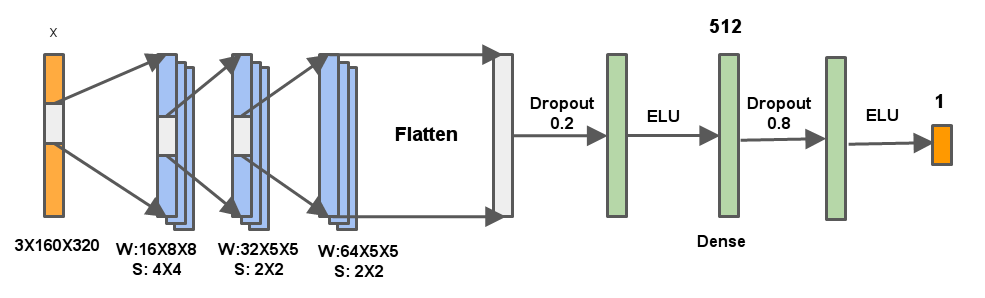
\includegraphics[width=\textwidth]{cnn}
    \caption{The Convolutional Neural Network architecture for feature extraction used in our work. The CNN model is based on the work by comma.ai}
    \label{fig:cnn}
\end{figure*}

\paragraph{}

\textbf{CNN Model:} As formulated in the above section, we can observe that the inputs to our model have varying dimensions. The image frame is $\mathbb{R}^{160\times320\times3}$ dimensional vector while the speed, brake, gas and gear position are $\mathbb{R}^{1\times1}$ dimensional vector. Therefore, we use a CNN model which take image frame as an input and give out a feature 512 dimensional feature vector. As, this will help in reducing the very high dimensional information into a comparatively low dimension. It also help in removing the redundant information and focus only on the useful features. Therefore, for the CNN model we used a 8 layer model including 3 convolutional layers each having 3X3 dimensional convolution kernel with a stride of 4 for cnn layer2, 2 for both cnn layer 4 and layer 6. The activation function used was ReLu while a dropout of 0.2 was used before the 512 dense feature vectors. \\


\begin{figure*}[ht]
    \center
    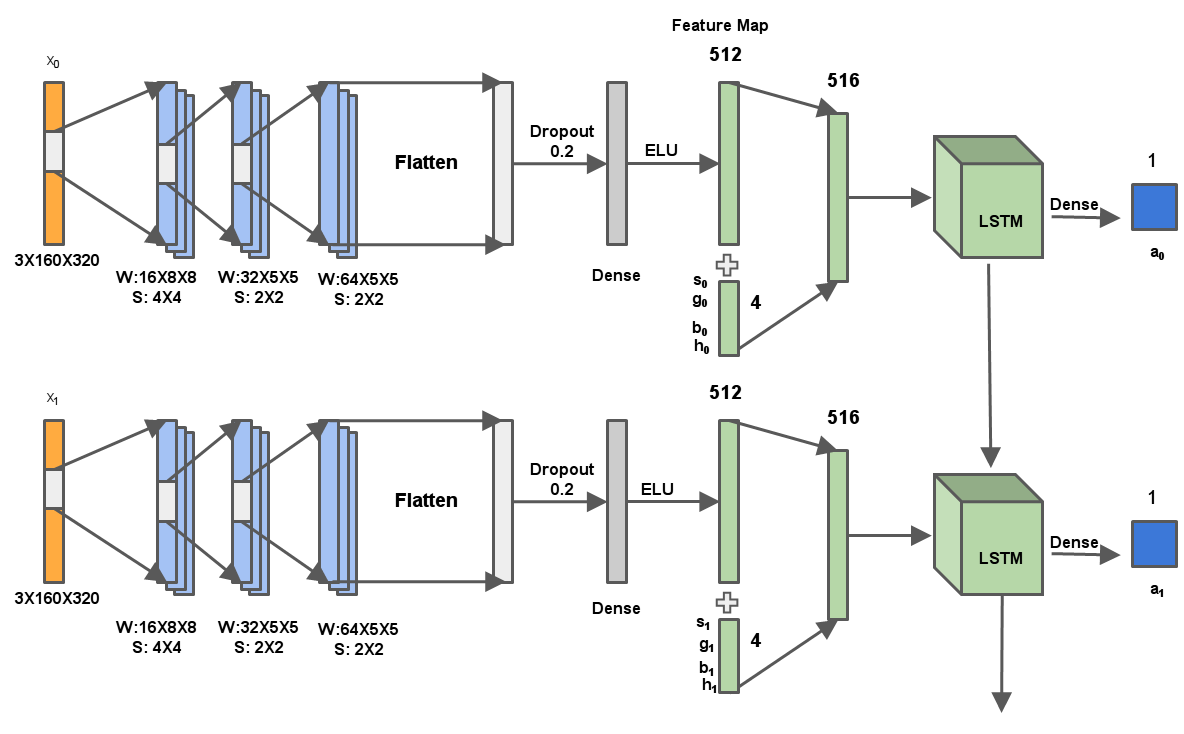
\includegraphics[width=\textwidth]{lrcn}
    \caption{The deep LRCN architecture used in our work. The CNN model is adopted from the above mentioned CNN model}
    \label{fig:figure1}
\end{figure*}

\textbf{LRCN Model:} It consists of CNN model which we have described earlier upto the 512 feature vector layer along with a LSTM model. As, driving states are sequential in nature and each state has temporal information. In order to extract the temporal relation, we added the values of brake, gas, speed and gear to the feature 512 feature vectors. Therefore, we now get 516 vectored element compressed information about the current state which will be then used for predicting the next generated command. In order to preserve the sequential information in the input, we use a LSTM model having 256 hidden layers which give a 1 dimensional dense output layer. The optimizer used for both the models is \emph{`adam'} while the loss is minimized on mean square error. \\

\textbf{Generative Model:} The generative model architecture is based on the work by \citeasnoun{comma} paper on Learning a Driver Simulator. We have used the main underlying idea and model proposed in the paper. The Encoder module use 4 convolution layer with each using batch norm followed by LeakyReLu activation function. The Generator model use 3 Deconvolution layers along with batch normalization after each layer with ReLu being used as an activation function. The 4th deconvolution layer uses tanh as activation function. Lastly, the discriminator model is pretty much similar to encoder model. The learning rate used is 0.0002.

%\begin{equation}
%L= - \frac{1}{N_{i}}\sum_{n=1}^{N_{i}}\bigg[ylog(a) + (1-y)log(1-a))\bigg]
%\end{equation}





\section{Experimental Result}
\subsection{Dataset}
The dataset  used in the project is taken from the the online release dataset from comma.ai. The dataset consists of 7.5 hours of driving on highways. It is divided into 11 sub-datasets where currently we are using 9 for training while other 2 for testing. The dataset is taken on Acura ILX 2016 using a Point Grey camera. All the datasets are interpolated to fit the sampling rate at 100 Hz. The sensor information include steering wheel, gear, gas pedal position, clutch, brake, radar, IMU, GPS, etc. The dataset image frames are classified as \emph{good} and \emph{not good} frames. Frames were steering angle is within 20 degrees are termed as \emph{good} while rest of other frames having steering angle greater than 20 degrees are treated as \emph{not good} frames. These data will be used for the ground truth comparison. The dataset is stored in HDF5 format which make it easy for python usage.

\begin{figure*}
    \center
    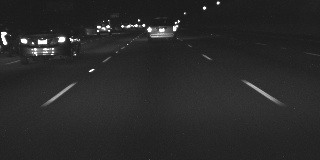
\includegraphics[width=\textwidth]{image}
    \caption{Sample image frame taken from dataset}
    \label{fig:figure6}
\end{figure*} 

Apart from commai.ai dataset, we are also using the datasets provided by Udacity . The dataset provided by Udacity is also taken on 2016 Lincoln MKZ. It uses 2 velodyne VLP-16 LiDARs, 1 Delpi radar, 3 Point Grey Blackfly cameras, an Xsens IMU, an ECU for sensor data collection. As it can be observed that both the datasets i.e. by comma.ai and Udacity were taken from same car, therefore, the trained model can easily be tested on the cross dataset. Apart from that we are also planning to use Kitty dataset in training and testing of the proposed model. 

\subsection{Training} 
\paragraph{}
\textbf{CNN Model Training:} Following the training methodology used by comma.ai, we tried to follow a similar approach towards training. The comma.ai's 11 video datasets were divided such that 9 were used for training while 2 were used for testing. The model was trained for 200 epochs with each epoch consisting of 10000 normalized frame of dimension $3\times160\times320$. Each epoch consisted of a batch size of 64 pertaining to the resource constraints. The whole model was trained on a Nvidia GT 740 GPU with 2Gbs of memory and 12 Gbs of RAM. The whole CNN model takes around 11 hours for training.\\

\textbf{LRCN Model Training:} For our LRCN model, we have used time distribution of CNN model where we used 4 CNN models in our time distributed model. Training of LRCN model is done in a divide and conquer principle with an iterative approach. As mentioned earlier, we already have our CNN model trained. Therefore, for training LSTM model we keep the CNN model weight unchanged and train the LSTM model on top of that for 20 epochs. Each epoch consists of 10000 frames with each epoch having batch size of 32. So, each batch consists of 32 sets of 4 consecutive frames sent to time distributed CNN model. Our output of the CNN model will be $\mathbb{R}^{4\times512\times1}$  vectored feature map which is concatenated with corresponding gas, gear, speed and brake position values to give a vector of dimension $\mathbb{R}^{4\times516\times1}$ which is sent to our LSTM model. The output of our model will be a single value scalar which is our objective for optimization.\\

\textbf{Generative Model Training:} Generative model training is consists of two phases of training. Initially, autoencoder module is trained at first for 200 epochs with each epoch having 10000 images in a batch of 32. During training, three consecutive training metadata is stored. Once the autoencoder module is trained, we then start training our transition model using RNN model. Each epoch takes approximately 5 minutes to train on GT 740.

\begin{figure}[H]
\centering
  \subfigure[Frame with label "Predicted vs Actual on a Straight road"]{\label{fig:steerangle:straight} {\setlength\fboxsep{0pt}\setlength\fboxrule{0pt}\fbox{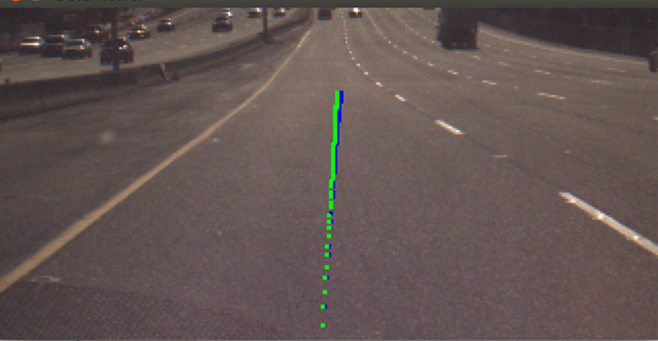
\includegraphics[height=0.25\textwidth]{straight}}}}
  \subfigure[Frame with label "Predicted vs Actual on a Curvy road"]{\label{fig:steerangle:curve} {\setlength\fboxsep{0pt}\setlength\fboxrule{0pt}\fbox{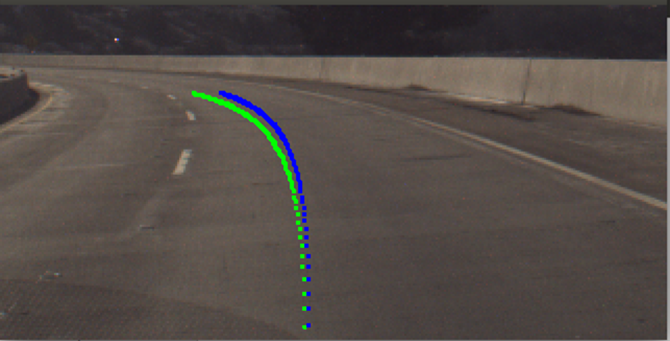
\includegraphics[height=0.25\textwidth]{curve}}}}
  \subfigure[Frame with label "Plot of Predicted vs Ground Truth on whole video dataset 10"]{\label{fig:steerangle:error_out1} {\setlength\fboxsep{0pt}\setlength\fboxrule{0pt}\fbox{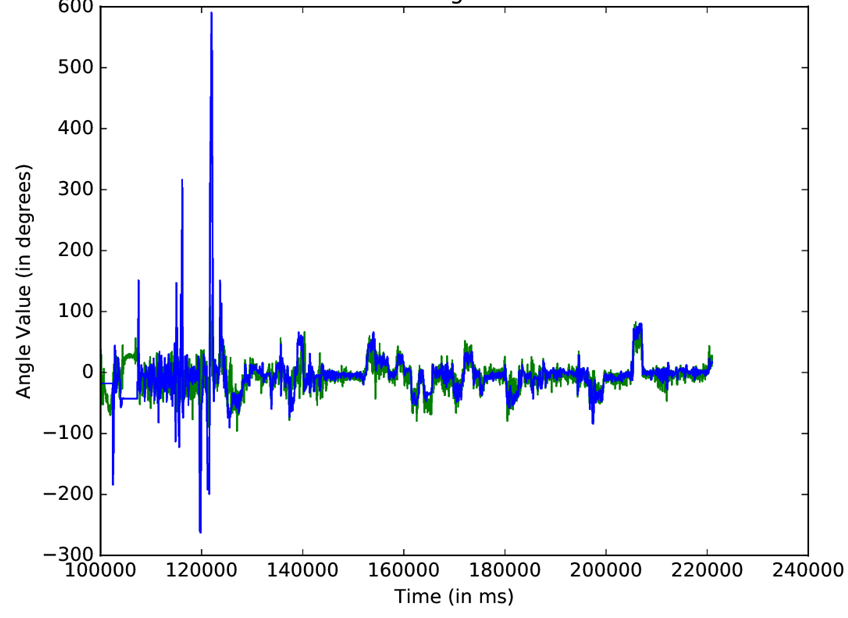
\includegraphics[height=0.33\textwidth]{error_out1}}}}
    \subfigure[Frame with label "Plot of Predicted vs Ground Truth on frame number 220000-223000 of video dataset 10"]{\label{fig:steerangle:error_out2} {\setlength\fboxsep{0pt}\setlength\fboxrule{0pt}\fbox{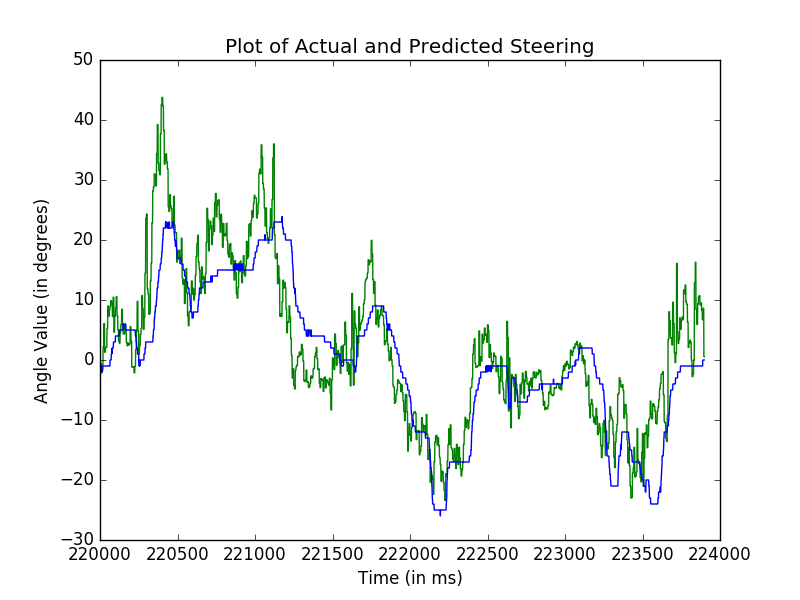
\includegraphics[height=0.37\textwidth]{error_out2}}}}
\caption{Comparison between predicted steering angle (green) vs ground truth (blue) for the video dataset 10 from comma.ai by our proposed model}
\label{fig:steerangle}
\end{figure}

\subsection{Evaluation}

\subsection*{Steering Angle}

To start with, we trained our model to predict steering angle. We tested our model on video dataset 10 and 11 given by comma.ai. Fig. 2 (a) and (b) show the predicted (green line) vs the ground truth (blue line) trajectory, and it can be inferred that both are quite close while the model has some problem predicting for curve lane as it shows more error. The predicted vs ground truth angle values for all frames of video dataset 10 is plotted as shown in Fig. 2(c) while Fig. 2(d) show the time zoomed version from the frames 224000-223000. It can be seen that the model is able to estimate the steering angle. Another inference can be drawn is that the model output has high frequency jittering.

%The performance of both networks is measured by the frame wise accuracy. The accuracy of frame based recognition network is $30.50\%$. The accuracy of space time volume based recognition network is $28.00\%$. 

\begin{figure}[]
\centering
  \subfigure[Frame with label "Output from Convolutional layer 1 "]{\label{fig:cnn_layer:cnn_layer1} {\setlength\fboxsep{0pt}\setlength\fboxrule{0pt}\fbox{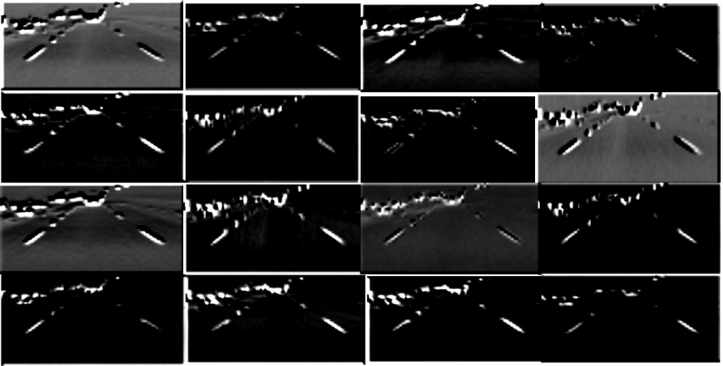
\includegraphics[height=0.50\textwidth]{cnn_layer1}}}}
  \subfigure[Frame with label "Output from Convolutional layer 2"]{\label{fig:cnn_layer:cnn_layer2} {\setlength\fboxsep{0pt}\setlength\fboxrule{0pt}\fbox{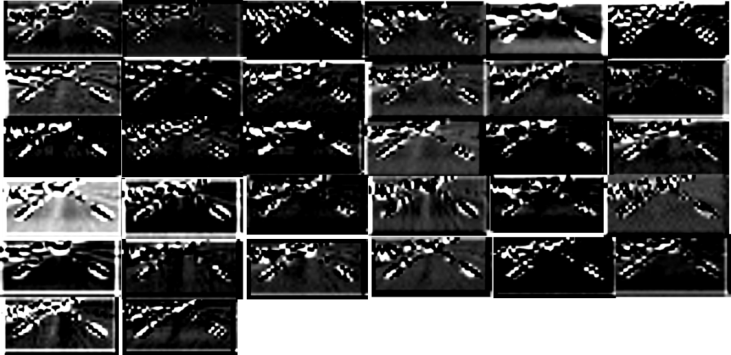
\includegraphics[height=0.49\textwidth]{cnn_layer2}}}} 
  \subfigure[Frame with label "Output from Convolutional layer 3"]{\label{fig:cnn_layer:cnn_layer3} {\setlength\fboxsep{0pt}\setlength\fboxrule{0pt}\fbox{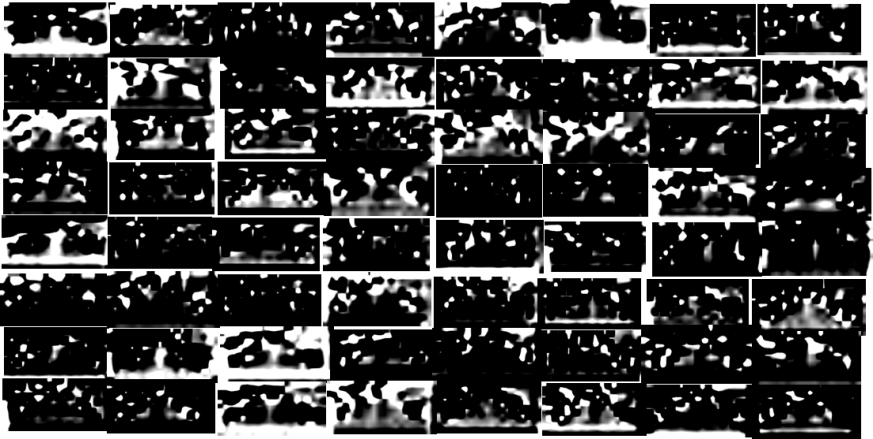
\includegraphics[height=0.50\textwidth]{cnn_layer3}}}}
\caption{Ouput of convolutional layers of the proposed model when a frame from video \emph{dataset} 10 was given to model as an input}
\label{fig:cnn_layer}
\end{figure}

\subsection*{Convolutional Layers Output}

Convolutional layers bring a hierarchical abstraction in the data and are output of each layers gives very critical information about the what the model is learning. Fig 3 (a), (b) and (c) show the output of convolutional layers 1, 2 and 3 respectively. It can be seen that the layer 1 learns highest level of abstraction where in some of output frames both right and left sides of lane are learnt. While, in Fig. 3(b) it can be seen that model learns lane centre, edges, boundary and other information which is hard to comprehend.

\subsection*{Generative Model Output}

Based on the work of comma.ai on using generative model for learning the transitions in the image frame, we used their designed model for training. We observed that the model is able to learn upto 100 frames. It works well for straight roads but has a problem modelling curvy roads and after few frames, the model always transitions from curvy road to straight one. Fig. 4 shows output of our generative model show learnt transitions. It can be seen that the learnt transition is blurred.

\begin{figure*}
    \center
    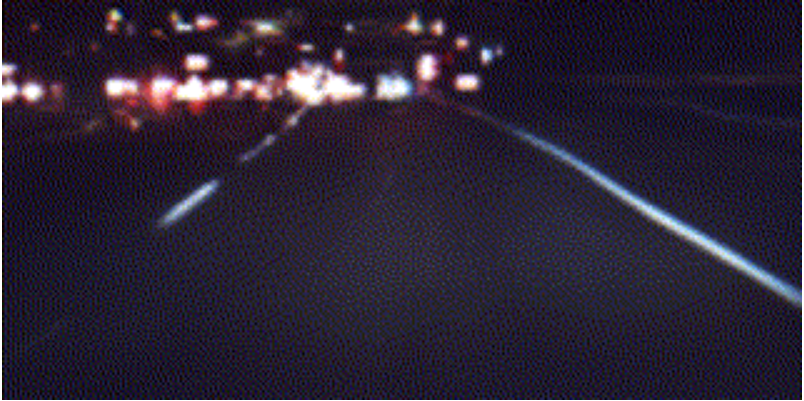
\includegraphics[width=\textwidth]{gan_out}
    \caption{Transition output of Generative Adversarial Network model}
    \label{fig:figure6}
\end{figure*}  


% CONCLUSIONS
\section{Future Work}

The model is trained for prediction of steering wheel till now and our next objective is to train the other driving parameters by the use of LRCN model. In our initial training of LRCN model, the model is having difficulty of learning the objective function. Therefore, we would like to see the effect of change in the number of feature vectors on the model prediction and relevant optimizations required in making the system robust towards modelling turns on road. Also, our initial work is based on estimation of steering wheel angle and plan to extend prediction of other driving parameters.

Our future work also includes improving on the generative model developed by comma.ai to make it work on curvy roads too. As discussed in earlier section that the developed model by comma.ai has difficulty in learning the transitions on a curvy road and after few frames it transits back to straight road. This problem arises due to unbalanced dataset i.e. majority of frames are for straight roads as the dataset was collected on highways. Therefore, we aim to improve the situation by training it on balanced dataset having an equal mix of both. This methodology was employed by Nvidia during their training of CNN model.


\section{Conclusion}

The work proposes a way using recent developments in deep learning to model complex driving behaviours and patterns in order to predict driving states using the dashboard mounted sensors on a car. The developed model uses convolutional neural network for converting image frame to feature vectors which models the spatial information and then LSTM to model the temporal information in the data in order to predict the gear, gas and break position in order. We used  open source publicly available datasets from comma.ai and udacity for training and testing of our model.


% REFERENCES
\addcontentsline{toc}{section}{References}
\small
\singlespacing
%\printbibliography[maxnames=99]
\bibliography{report}
\bibliographystyle{ieeetr}


\end{document}
